\documentclass[11pt,a4paper]{article}

% --- Kötelező és alapvető csomagok ---
\usepackage[utf8]{inputenc}
\usepackage[T1]{fontenc}
\usepackage[magyar]{babel}
\usepackage{amsmath, amssymb, amsthm}
\usepackage[margin=2cm]{geometry}
\usepackage{xcolor}
\usepackage[most]{tcolorbox}
\usepackage{tikz}
\usepackage{multicol}
\usepackage{enumitem}
\usepackage{microtype}

%%% Megjelenítéshez automatikusan kiegészített csomagok %%%
\usepackage{pgfplots}
\pgfplotsset{compat=1.18}
\usepackage{graphicx}
\usepackage{booktabs}
\usepackage{float}
\usepackage{caption}

\usepackage{hyperref}

% --- Színpaletta meghatározása ---
\definecolor{primaryBlue}{RGB}{20, 60, 110}
\definecolor{secondaryTeal}{RGB}{0, 130, 130}
\definecolor{accentOrange}{RGB}{210, 85, 20}
\definecolor{lightBg}{RGB}{248, 250, 252}
\definecolor{darkGray}{RGB}{50, 50, 50}

% --- TColorBox sablonok kialakítása ---
\tcbuselibrary{skins, breakable}

% Definíció doboz
\newtcolorbox{definrans}[1]{
    colback=lightBg,
    colframe=secondaryTeal,
    fonttitle=\bfseries\sffamily,
    coltitle=white,
    title={Definíció: #1},
    enhanced,
    sharp corners,
    attach boxed title to top left={yshift=-2mm, xshift=4mm},
    boxed title style={sharp corners, colback=secondaryTeal},
    top=4mm, bottom=3mm, left=3mm, right=3mm,
    boxrule=0.8pt,
    drop shadow=black!10
}

% Tétel doboz
\newtcolorbox{tetelbox}[1]{
    colback=lightBg,
    colframe=primaryBlue,
    fonttitle=\bfseries\sffamily,
    coltitle=white,
    title={Tétel: #1},
    enhanced,
    sharp corners,
    attach boxed title to top left={yshift=-2mm, xshift=4mm},
    boxed title style={sharp corners, colback=primaryBlue},
    top=4mm, bottom=3mm, left=3mm, right=3mm,
    boxrule=0.8pt,
    drop shadow=black!10
}

% Kidolgozott példa doboz
\newtcolorbox{peldabox}[1]{
    colback=white,
    colframe=accentOrange,
    fonttitle=\bfseries\sffamily,
    coltitle=white,
    title={Mintapélda: #1},
    enhanced,
    sharp corners,
    attach boxed title to top left={yshift=-2mm, xshift=4mm},
    boxed title style={sharp corners, colback=accentOrange},
    top=4mm, bottom=3mm, left=3mm, right=3mm,
    boxrule=0.8pt,
    drop shadow=black!10,
    breakable
}

% Megjegyzés / Fontos kiemelés
\newtcolorbox{fontosbox}{
    colback=accentOrange!5,
    colframe=accentOrange!80!black,
    boxrule=0pt,
    leftrule=3.5pt,
    arc=0mm,
    fonttitle=\bfseries\color{accentOrange!80!black},
    title={Fontos megjegyzés:},
    top=2mm, bottom=2mm, left=3mm, right=3mm
}

\setlength{\parindent}{0pt}
\setlength{\parskip}{6pt}

\begin{document}

% --- Fejléc és Cím ---
\begin{center}
    {\scshape\Large Középiskolai Matematika Összefoglaló}\\[0.2cm]
    {\Huge\bfseries\color{primaryBlue} Másodfokú egyenletek és a diszkrimináns}\\[0.3cm]
    \rule{0.8\textwidth}{1.5pt}
\end{center}

\vspace{0.2cm}

\section{Alapfogalmak és típusok}

A másodfokú egyenletek a középiskolai algebra egyik legfontosabb sarokkövét képezik. Számos geometriai, fizikai és gazdasági probléma visszavezethető rájuk.

\begin{definrans}{Egyismeretlenes másodfokú egyenlet}
    Egyismeretlenes másodfokú egyenletnek nevezzük az olyan egyenletet, amely ekvivalens átalakításokkal az alábbi alakra hozható:
    \begin{equation}
        ax^2 + bx + c = 0 \quad (a, b, c \in \mathbb{R}, \, a \neq 0)
    \end{equation}
    Ahol:
    \begin{itemize}[noitemsep,topsep=0pt]
        \item $a$: a másodfokú tag együtthatója (főegyüttható),
        \item $b$: az elsőfokú (lineáris) tag együtthatója,
        \item $c$: a konstans tag (szabadtag).
    \end{itemize}
\end{definrans}

\subsection{Hiányos másodfokú egyenletek}
Amennyiben a $b$ vagy $c$ paraméter értéke $0$, hiányos másodfokú egyenletről beszélünk. Ezek megoldásához nincs szükség az általános megoldóképletre:
\begin{enumerate}[leftmargin=*]
    \item \textbf{Ha $b = 0$ és $c \neq 0$ ($ax^2 + c = 0$):} Tiszta másodfokú egyenlet. Rendezzük: $x^2 = -\frac{c}{a}$.
    \begin{itemize}[noitemsep]
        \item Ha $-\frac{c}{a} > 0$, akkor két valós megoldás van: $x_{1,2} = \pm \sqrt{-\frac{c}{a}}$.
        \item Ha $-\frac{c}{a} < 0$, a valós számok halmazán nincs megoldás.
    \end{itemize}
    \item \textbf{Ha $c = 0$ és $b \neq 0$ ($ax^2 + bx = 0$):} Kiemeléssel szorzattá alakítunk: $x(ax + b) = 0$. Egy szorzat akkor és csak akkor nulla, ha legalább az egyik tényezője nulla:
    \[
        x_1 = 0 \quad \text{vagy} \quad ax + b = 0 \implies x_2 = -\frac{b}{a}.
    \]
\end{enumerate}

\section{A megoldóképlet és a diszkrimináns}

\begin{tetelbox}{A másodfokú egyenlet megoldóképlete}
    Az $ax^2 + bx + c = 0$ ($a \neq 0$) egyenlet valós megoldásai:
    \begin{equation}
        x_{1,2} = \frac{-b \pm \sqrt{b^2 - 4ac}}{2a}
    \end{equation}
\end{tetelbox}

\begin{proof}[\textbf{Bizonyítás (Teljes négyzetté kiegészítéssel)}]
    Osszuk el az egyenlet mindkét oldalát $a$-val ($a \neq 0$):
    \[
        x^2 + \frac{b}{a}x + \frac{c}{a} = 0
    \]
    Egészítsük ki teljes négyzetté a bal oldalt az $(x+y)^2 = x^2 + 2xy + y^2$ azonosság alapján:
    \[
        \left(x + \frac{b}{2a}\right)^2 - \left(\frac{b}{2a}\right)^2 + \frac{c}{a} = 0
    \]
    Rendezzük az állandó tagokat a jobb oldalra, és hozzuk közös nevezőre:
    \[
        \left(x + \frac{b}{2a}\right)^2 = \frac{b^2}{4a^2} - \frac{c}{a} = \frac{b^2 - 4ac}{4a^2}
    \]
    Feltéve, hogy a számláló nem negatív, vonjunk négyzetgyököt mindkét oldalból:
    \[
        x + \frac{b}{2a} = \pm \frac{\sqrt{b^2 - 4ac}}{2a} \implies x_{1,2} = \frac{-b \pm \sqrt{b^2 - 4ac}}{2a}
    \]
\end{proof}

\begin{definrans}{A másodfokú egyenlet diszkriminánsa}
    A megoldóképlet gyök alatti kifejezését az egyenlet \textbf{diszkriminánsának} nevezzük, jele: $D$.
    \begin{equation}
        D = b^2 - 4ac
    \end{equation}
\end{definrans}

\subsection{A diszkrimináns szerepe és geometriai jelentése}

A valós gyökök száma kizárólag a diszkrimináns előjelétől függ:
\begin{itemize}[leftmargin=*]
    \item \textbf{$D > 0$:} Az egyenletnek \textbf{két különböző valós gyöke} van ($x_1 \neq x_2$). A megfelelő $f(x) = ax^2 + bx + c$ függvény grafikonja (parabola) \textbf{két pontban metszi} az $x$-tengelyt.
    \item \textbf{$D = 0$:} Az egyenletnek \textbf{egy valós gyöke} van (kettős gyök: $x_1 = x_2 = -\frac{b}{2a}$). A parabola csúcspontja az $x$-tengelyen fekszik, vagyis a görbe \textbf{érinti} az $x$-tengelyt.
    \item \textbf{$D < 0$:} Az egyenletnek a valós számok halmazán \textbf{nincs megoldása}. A parabola \textbf{nem metszi és nem érinti} az $x$-tengelyt (teljesen alatta vagy felette halad).
\end{itemize}

\begin{center}
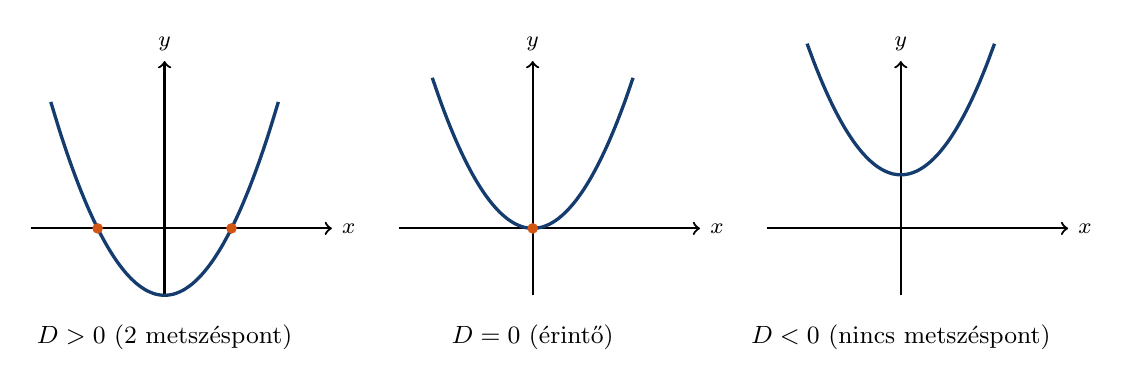
\begin{tikzpicture}[scale=0.85]
    % Ábra 1: D > 0
    \begin{scope}[shift={(0,0)}]
        \draw[->, thick] (-2,0) -- (2.5,0) node[right] {\footnotesize $x$};
        \draw[->, thick] (0,-1) -- (0,2.5) node[above] {\footnotesize $y$};
        \draw[domain=-1.7:1.7, smooth, variable=\x, primaryBlue, line width=1.2pt] 
            plot ({\x}, {\x*\x - 1});
        \filldraw[accentOrange] (-1,0) circle (2pt);
        \filldraw[accentOrange] (1,0) circle (2pt);
        \node[below] at (0,-1.3) {\small $D > 0$ (2 metszéspont)};
    \end{scope}

    % Ábra 2: D = 0
    \begin{scope}[shift={(5.5,0)}]
        \draw[->, thick] (-2,0) -- (2.5,0) node[right] {\footnotesize $x$};
        \draw[->, thick] (0,-1) -- (0,2.5) node[above] {\footnotesize $y$};
        \draw[domain=-1.5:1.5, smooth, variable=\x, primaryBlue, line width=1.2pt] 
            plot ({\x}, {\x*\x});
        \filldraw[accentOrange] (0,0) circle (2pt);
        \node[below] at (0,-1.3) {\small $D = 0$ (érintő)};
    \end{scope}

    % Ábra 3: D < 0
    \begin{scope}[shift={(11,0)}]
        \draw[->, thick] (-2,0) -- (2.5,0) node[right] {\footnotesize $x$};
        \draw[->, thick] (0,-1) -- (0,2.5) node[above] {\footnotesize $y$};
        \draw[domain=-1.4:1.4, smooth, variable=\x, primaryBlue, line width=1.2pt] 
            plot ({\x}, {\x*\x + 0.8});
        \node[below] at (0,-1.3) {\small $D < 0$ (nincs metszéspont)};
    \end{scope}
\end{tikzpicture}
\end{center}

\section{Gyöktényezős alak és a Viète-formulák}

\begin{tetelbox}{Gyöktényezős alak}
    Ha az $ax^2 + bx + c = 0$ egyenlet valós gyökei $x_1$ és $x_2$, akkor a másodfokú polinom szorzattá alakítható:
    \begin{equation}
        ax^2 + bx + c = a(x - x_1)(x - x_2)
    \end{equation}
\end{tetelbox}

\begin{tetelbox}{Viète-formulák (Gyökök és együtthatók kapcsolata)}
    Ha az $ax^2 + bx + c = 0$ egyenlet gyökei $x_1$ és $x_2$, akkor a gyökök összege és szorzata kifejezhető az együtthatókkal:
    \begin{equation}
        x_1 + x_2 = -\frac{b}{a} \qquad \text{és} \qquad x_1 \cdot x_2 = \frac{c}{a}
    \end{equation}
\end{tetelbox}

\section{Kidolgozott mintapéldák}

\begin{peldabox}{1. feladat: Teljes másodfokú egyenlet megoldása}
    \textbf{Feladat:} Oldjuk meg az alábbi egyenletet a valós számok halmazán!
    \[
        2x^2 - 5x - 3 = 0
    \]
    \textbf{Megoldás:}\\
    1. Azonosítsuk az együtthatókat: $a = 2$, $b = -5$, $c = -3$.\\
    2. Számítsuk ki a diszkriminánst:
    \[
        D = b^2 - 4ac = (-5)^2 - 4 \cdot 2 \cdot (-3) = 25 + 24 = 49
    \]
    Mivel $D > 0$, így két valós megoldás létezik, és $\sqrt{D} = \sqrt{49} = 7$.\\
    3. Helyettesítsünk a megoldóképletbe:
    \[
        x_{1,2} = \frac{-(-5) \pm 7}{2 \cdot 2} = \frac{5 \pm 7}{4}
    \]
    Ebből a két gyök:
    \[
        x_1 = \frac{5 + 7}{4} = \frac{12}{4} = 3, \qquad x_2 = \frac{5 - 7}{4} = \frac{-2}{4} = -\frac{1}{2}
    \]
    \textbf{Ellenőrzés Viète-formulákkal:}
    $x_1 + x_2 = 3 - \frac{1}{2} = \frac{5}{2} = -\frac{b}{a}$, és $x_1 \cdot x_2 = 3 \cdot \left(-\frac{1}{2}\right) = -\frac{3}{2} = \frac{c}{a}$. A megoldás helyes.
\end{peldabox}

\begin{peldabox}{2. feladat: Paraméteres egyenlet vizsgálata diszkriminánssal}
    \textbf{Feladat:} Határozzuk meg a $p$ valós paraméter értékét úgy, hogy az alábbi egyenletnek pontosan egy valós gyöke legyen!
    \[
        x^2 - 2(p - 1)x + (2p + 1) = 0
    \]
    \textbf{Megoldás:}\\
    Egy másodfokú egyenletnek akkor és csak akkor van pontosan egy valós gyöke, ha diszkriminánsa nulla ($D = 0$).\\
    Az együtthatók: $a = 1$, $b = -2(p-1)$, $c = 2p + 1$.
    \begin{align*}
        D = b^2 - 4ac &= \left[-2(p-1)\right]^2 - 4 \cdot 1 \cdot (2p + 1) \\
        &= 4(p^2 - 2p + 1) - 8p - 4 \\
        &= 4p^2 - 8p + 4 - 8p - 4 = 4p^2 - 16p
    \end{align*}
    A feltétel szerint $D = 0$:
    \[
        4p^2 - 16p = 0 \implies 4p(p - 4) = 0
    \]
    A szorzat nulla, ha $p_1 = 0$ vagy $p_2 = 4$.\\
    \textbf{Válasz:} Az egyenletnek $p = 0$ vagy $p = 4$ esetén van pontosan egy valós gyöke.
\end{peldabox}

\section{Önálló gyakorló feladatok}

Oldd meg az alábbi feladatokat a füzetedben!

\begin{enumerate}[label=\textbf{\arabic*.}]
    \item Oldd meg a valós számok halmazán a következő hiányos másodfokú egyenleteket!
    \begin{multicols}{2}
        \begin{enumerate}[label=\alph*)]
            \item $3x^2 - 27 = 0$
            \item $5x^2 + 20x = 0$
        \end{enumerate}
    \end{multicols}

    \item Határozd meg a valós megoldásokat a megoldóképlet segítségével!
    \begin{multicols}{2}
        \begin{enumerate}[label=\alph*)]
            \item $x^2 - 8x + 15 = 0$
            \item $3x^2 + 2x - 1 = 0$
        \end{enumerate}
    \end{multicols}

    \item Számítsd ki a diszkriminánst, és döntsd el a valós gyökök számát a képlet alkalmazása nélkül!
    \begin{multicols}{2}
        \begin{enumerate}[label=\alph*)]
            \item $2x^2 - 4x + 5 = 0$
            \item $4x^2 - 12x + 9 = 0$
        \end{enumerate}
    \end{multicols}

    \item \textbf{Emelt szintű kihívás:} A gyökök kiszámítása nélkül írj fel olyan másodfokú egyenletet, amelynek gyökei az $x^2 - 7x + 10 = 0$ egyenlet gyökeinek kétszeresei!
\end{enumerate}

\begin{fontosbox}
Mindig ellenőrizd az értelmezési tartományt törtes vagy gyökös kifejezésekre visszavezethető egyenleteknél, és ne feledkezz meg a gyökök ellenőrzéséről behelyettesítéssel vagy Viète-formulákkal!
\end{fontosbox}

\vspace{0.4cm}
\hrule
\vspace{0.2cm}
{\footnotesize \textbf{Végeredmények az önellenőrzéshez:}\\
1. a) $x_{1,2} = \pm 3$; \quad b) $x_1 = 0, \, x_2 = -4$ \qquad
2. a) $x_1 = 3, \, x_2 = 5$; \quad b) $x_1 = \frac{1}{3}, \, x_2 = -1$\\
3. a) $D = -24 < 0 \implies 0$ valós gyök; \quad b) $D = 0 \implies 1$ valós gyök\\
4. Az új egyenlet: $x^2 - 14x + 40 = 0$}

\end{document}